The Data Management System (DMS) is responsible for the communication with third-party flight data APIs. It allows the request of flight data in behalf of the CSA. This implementation of the DMS is based on a low-level API wrapper, around the KIWI flight API, and it is constructed as a worker/consumer factory to execute concurrent HTTP requests (see figure \ref{fig:dms_implementation}). 

%As discussed in section \ref{sec:dms_design}, it is possible to obtain this flight data in two distint ways, by using a third-party flight data API, or by performing web scraping. Both of these methods were implemented and tested, and the results will be discussed in section \textbf{put the section  of the comparison of API vs webscraping here}. During the development of this work, several API's were tested, and the one which is currently being used is the \textit{Kiwi.com} API, whose details can be found in the followig website: \textit{https://docs.kiwi.com/}. 

Given a list of necessary flights, usually requested by the CSA, the DMS communicates with third-party APIs as to request the relevant flight data. This communication relies on the HTTP protocol, and uses the URI as to identify a particular resource. This identification follows the protocol defined by the third-party API \cite{kiwi_api}. A response to a request is given by a structured data tree, usually as a JSON data type. Hence, each worker of the DMS worker/consumer factory executes the following tasks:
\begin{enumerate}
  \item generate the URL for the intended resource;
  \item execute an HTTP request to the given URL;
  \item parse the response.
\end{enumerate}

When communicating with third-party APIs, the bottleneck of the system is usually the time necessary for the server to process the request and produce a response to it. The implemented worker/consumer approach takes advantage of this bottleneck. Instead of waiting for a request to complete, this approach uses the waiting period to spawn more requests. Thus, the waiting period associated to one request is not imposed to the others. Despite this, executing multiple requests will increment the servers workload, increasing the time necessary to respond to one (isolated) request. This approach will be discussed, and its results illustrated, in subsection \ref{sec:response_time}. 


%The worker/consumer approach implemented by this DMS is particularly useful to take advantage of the bottleneck of the communica


%Communicating with a third-party API to request flight data is simply a matter of making HTTP requests using an URL which defines the resource under query. This request is usually answered with a JSON or XML object, which contains the relevant response for the performed request. In general, each API has its own URL syntax and response structure. Thus, communicating with different API's requires the differentiation of the resource identification and response parsing methods, because these are usually API dependent. 


%These three essential steps are the base for any data collection system. They can be used to collect data from an API, and they can also be used to do webscraping. In general, the difference between these two methods (api vs webscraping) is more likely to be felt in the parsing of the response. Using an API, the response is usually structured and organized, encoded in a JSON data type, or similar,which is, in general, human readable. In its turn, using web scraping, the response comes in the form of HTML, and the necessary data may be trapped under many levels of HTML objects. In general, it is harder to parse the result of webscraping.

%There is a second difference that must be mentioned when comparing the usage of API's and webscraping. Webscraping is the act of retrieving the data visible on the \textit{screen}. The problem is that, in many cases, before the data becomes visable,  javascript has to be executed, and in some cases, there are database acceses, which usually require a substaintial ammoun of time to execute. In this case, it is said that the websites uses javascript to render their page, and in general, webscraping javascript websites is much more harder and slower, because a simple HTTP request is not sufficient to obtain the necessary data. Instead, it is necessary to emulate a browser, make the HTTP request, and wait for the javascript to be completly loaded. During the development of this system, the \textit{httplib} module of the python programming language was utilized for executing the HTTP requests, and the \textit{Selenium Web driver} library for the execution of a automatable browser.

%Given a list of flights whose data must be collected, figure \ref{fig:serial_api} illustrates the necessary steps to communicate  with a thid-party API, using HTTP protocol, to obtain the necessary data. In this figure, the system utilizes a serial approach, which means that at any time, only one request is being executed. 

%\todo{Esta imagem sera revista}
%\begin{figure}[htpb]
%  \centering
%  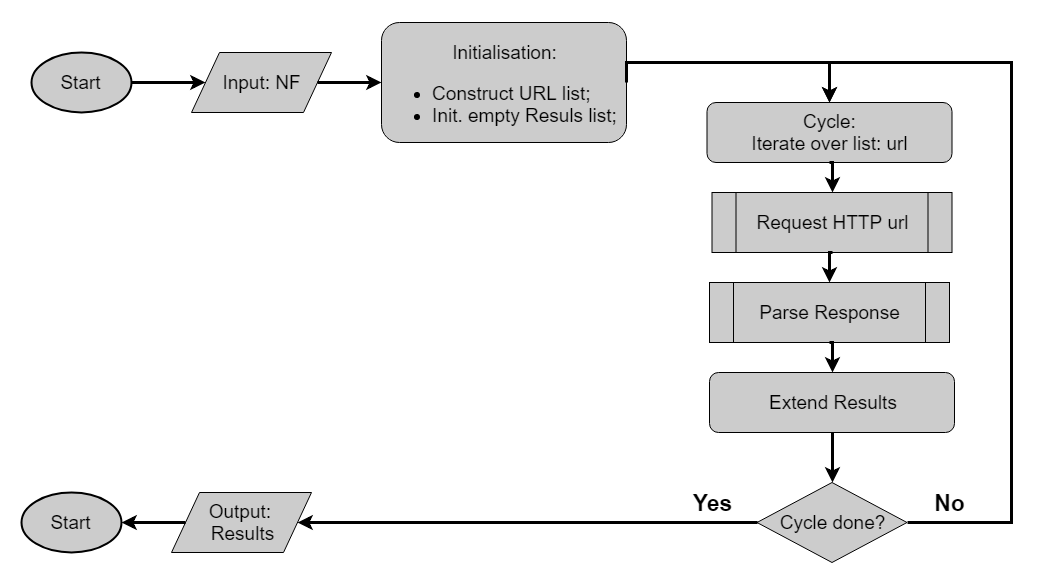
\includegraphics[width=\textwidth]{./Figures/system_implementation/serial_api.png}
%  \caption{Communication with third-party API's, using HTTP protocol, and a serial requesting scheme.}
%  \label{fig:serial_api}  
%\end{figure}

%The bottleneck of the serial system illustrated in figure \ref{fig:serial_api}, is the necessary time to receive the response to an HTTP request. In order to take advantage of this bottleneck, a concurrent approach was considered, in which the waiting period of a request is utilized to spwan more requests. This approach is achieved by adopting a \textit{Producer-Consumer} system, illustrated in figure \ref{fig:concurrent_api}. This system spwans at most $n_{max}$ threads (workers), one at a time, to execute a list of jobs, which correspond to making an HTTP request and parsing the response. Using this approach, the bottleneck experienced by each worker is not imposed on any of the other $n_{max} -1$ workers, and thus the time-delay is not cummulative.


\begin{figure}[h]
  \centering
  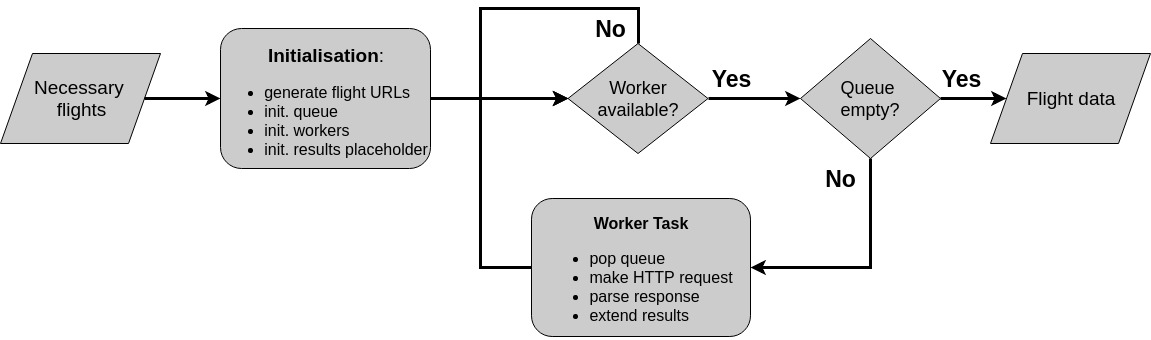
\includegraphics[width=\textwidth]{./Figures/system_implementation/dms_factory.jpg}
  \caption{The Data Management System uses concurrent HTTP requests to communicate with third-party flight API's.}
  \label{fig:dms_implementation}  
\end{figure}

%\begin{figure}[htpb]
%  \centering
%  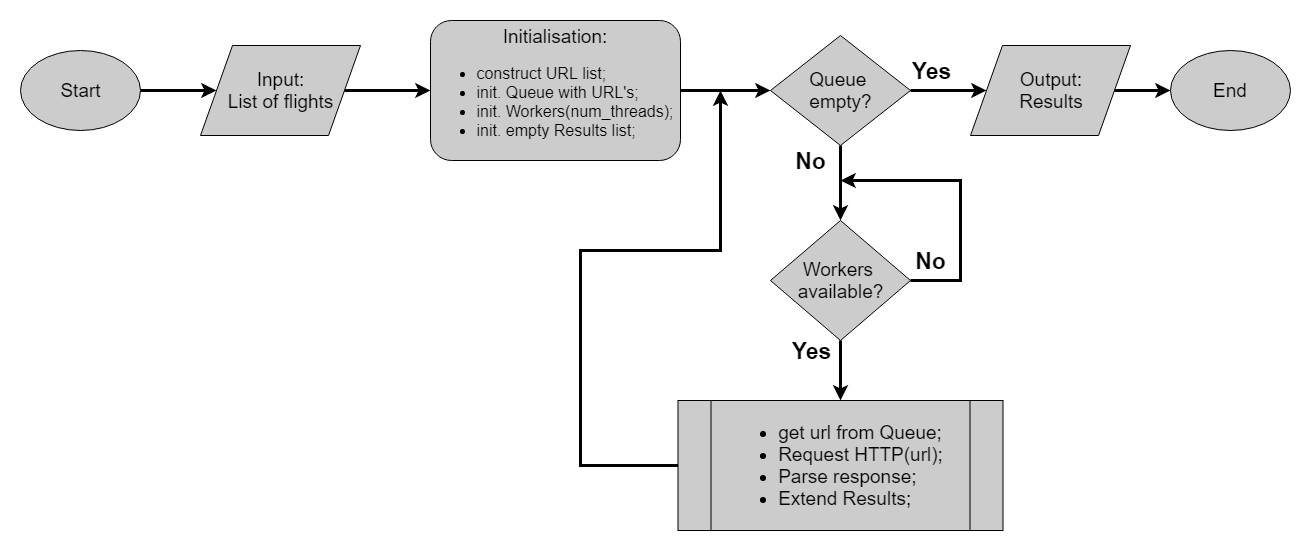
\includegraphics[width=\textwidth]{./Figures/system_implementation/concurrent_api.png}
%  \caption{Communication with third-party API's, using HTTP protocol, and concurrent requesting scheme to take advantage of the waiting times.}
%  \label{fig:concurrent_api}  
%\end{figure}


% The webscraping systems developed are very similar to those illustrated in figures \ref{fig:serial_api} and \ref{fig:concurrent_api}. However, instead of making simple HTTP requests, a Selenium browser is used to access the website. Consequentially, the execution of the concurrent approach must create, at most, $n_{max}$ browsers. The illustration of these systems may be consulted in the \textbf{ANEXO}.

%Subsection \textbf{section herereeere} will evaluate the proposed system, and compare the efficiency of the serial and concurrent approaches, for both the API collectiong and the webscraping. These two systems will also be compared in order to evaluate which is most adequate for the usage in a production system.



